\documentclass[10pt, landscape]{article}
\usepackage[scaled=0.92]{helvet}
\usepackage{calc}
\usepackage{multicol}
\usepackage[a4paper,margin=3mm,landscape]{geometry}
\usepackage{amsmath,amsthm,amsfonts,amssymb}
\usepackage{color,graphicx,overpic}
\usepackage{hyperref}
\usepackage{newtxtext} 
\usepackage{enumitem}
\usepackage[table]{xcolor}
\usepackage{mathtools}
\setlist{nosep}
% for including images
\graphicspath{ {./images/} }

\pdfinfo{
  /Title (springboot.pdf)
  /Creator (TeX)
  /Producer (pdfTeX 1.40.0)
  /Author (Tan Ping Zhi)
  /Subject (CSIT)
/Keywords (springboot, nus,cheatsheet,pdf)}

% Turn off header and footer
\pagestyle{empty}

% redefine section commands to use less space
\makeatletter
\renewcommand{\section}{\@startsection{section}{1}{0mm}%
  {-1ex plus -.5ex minus -.2ex}%
  {0.5ex plus .2ex}%x
{\normalfont\large\bfseries}}
\renewcommand{\subsection}{\@startsection{subsection}{2}{0mm}%
  {-1explus -.5ex minus -.2ex}%
  {0.5ex plus .2ex}%
{\normalfont\normalsize\bfseries}}
\renewcommand{\subsubsection}{\@startsection{subsubsection}{3}{0mm}%
  {-1ex plus -.5ex minus -.2ex}%
  {1ex plus .2ex}%
{\normalfont\small\bfseries}}%
\makeatother

\renewcommand{\familydefault}{\sfdefault}
\renewcommand\rmdefault{\sfdefault}
%  makes nested numbering (e.g. 1.1.1, 1.1.2, etc)
\renewcommand{\labelenumii}{\theenumii}
\renewcommand{\theenumii}{\theenumi.\arabic{enumii}.}
\renewcommand\labelitemii{•}
\renewcommand\labelitemiii{•}

\definecolor{mathblue}{cmyk}{1,.72,0,.38}
\everymath\expandafter{\the\everymath \color{mathblue}}

% Don't print section numbers
\setcounter{secnumdepth}{0}

\setlength{\parindent}{0pt}
\setlength{\parskip}{0pt plus 0.5ex}
%% adjust spacing for all itemize/enumerate
\setlength{\leftmargini}{0.5cm}
\setlength{\leftmarginii}{0.5cm}
\setlist[itemize,1]{leftmargin=2mm,labelindent=1mm,labelsep=1mm}
\setlist[itemize,2]{leftmargin=4mm,labelindent=1mm,labelsep=1mm}
\setlist[itemize,3]{leftmargin=4mm,labelindent=1mm,labelsep=1mm}

% adding my commands
% tightcenter
\newenvironment{tightcenter}{%
  \setlength\topsep{0pt}
  \setlength\parskip{0pt}
  \begin{center}
    }{%
  \end{center}
}

% boxed
\newenvironment{tightbox}{%
  \setlength\topsep{0pt}
  \setlength\parskip{0pt}
  \begin{center}
    \begin{tabular}{|@{\hspace{\dimexpr\fboxsep+0.5\arrayrulewidth}}c@{\hspace{\dimexpr\fboxsep+0.5\arrayrulewidth}}|}
      \hline
    }
    {%
    \\ \hline
    \end{tabular}
  \end{center}
}

% fixed width box
\newenvironment{fixedbox}[1][0.7]{
  \setlength\topsep{0pt}
  \setlength\parskip{0pt}
  \begin{center}
    \begin{tabular}{|>{\centering\arraybackslash}m{#1\linewidth}|}
    \hline
  }{
  \\ \hline
  \end{tabular}
  \end{center}
}

% definition of a new term
\usepackage{soul}
\definecolor{paleyellow}{RGB}{251,243,218}
\newcommand{\definition}[2][]{\sethlcolor{paleyellow}\hl{\textbf{#2}} #1  $\rightarrow$}
% inline definition
\newcommand{\ildefinition}[1]{\sethlcolor{paleyellow}\hl{\textbf{#1}}}

% important note (attention)
\newcommand{\attention}{{\color{red}\textbf{! }}}

% nice proof
\newenvironment{niceproof}[1][Proof]
{%
  \sbox0{\textit{#1}. }%
  \list{}{\labelwidth\wd0 \leftmargin\wd0 \labelsep 0pt }
\item[\usebox0]}
  {\endlist}


\usepackage{color, soul}
\usepackage{listings}
\usepackage{inconsolata}

\definecolor{codegreen}{rgb}{0,0.6,0}
\definecolor{codegray}{rgb}{0.5,0.5,0.5}
\definecolor{codepurple}{HTML}{C42043}
\definecolor{backcolour}{HTML}{F2F2F2}
\definecolor{bookColor}{cmyk}{0,0,0,0.90}

\newcommand{\code}[1]{\texttt{\sethlcolor{backcolour}\hl{$\,$#1$\,$}}}

% SQL code blocks
% define SQL styles
\lstdefinestyle{mySQL}{%
  language=SQL,
  backgroundcolor=\color{backcolour},
  commentstyle=\color{codegreen},
  keywordstyle=\color{codepurple},
  numberstyle=\numberstyle,
  stringstyle=\color{codepurple},
  basicstyle=\scriptsize\ttfamily,
  breaklines=true,
}

\DeclareMathOperator{\pairwisemax}{pairwise-max}

\definecolor{myred}{rgb}{1,0,0} % RGB color model
\newcommand{\hlred}[1]{{\sethlcolor{myred}\hl{#1}}}

% -----------------------------------------------------------------------

\begin{document}
\raggedright
\footnotesize
\begin{multicols*}{2}
    % multicol parameters
    \setlength{\columnseprule}{0.25pt}

    \begin{center}
        \fbox{%
        \parbox{0.8\linewidth}{\centering \textcolor{black}{
            {\Large\textbf{Week 1}}
            \\ \normalsize{CSIT 2024}}
        \\ {\footnotesize \textcolor{gray}{github/TanPingZhi}}
        }%
        }
    \end{center}

    \section{pom.xml}
    \begin{itemize}
        \item Add this dependency into the pom.xml file to use Apache Tika
    \end{itemize}
    \begin{verbatim}
<dependency>
    <groupId>org.apache.tika</groupId>
    <artifactId>tika-parsers</artifactId>
    <version>1.17</version>
</dependency>
    \end{verbatim}

    \section{index.html}
    \begin{verbatim}
<!DOCTYPE html>
<html xmlns:th="http://www.thymeleaf.org">
<head>
    <title>Upload PDF</title>
</head>
<body>
<h1>Upload a PDF file</h1>
<form method="POST" enctype="multipart/form-data" action="/upload">
    <input type="file" name="file" accept="application/pdf"/>
    <button type="submit">Upload</button>
</form>

<div>
    <h2>PDF Content</h2>
    <pre th:text="${pdfContent}"></pre>
</div>
</body>
</html>

\end{verbatim}

    \begin{itemize}
        \item \hl{xlmns:th} is a namespace declaration for Thymeleaf
              \begin{itemize}
                  \item \hl{th} any attribute that starts with \hl{th:} is a Thymeleaf attribute
                  \item Thymeleaf is a modern server-side Java template engine for both web and standalone environments.
              \end{itemize}
    \end{itemize}


    \section{PdfController.java}
    \begin{verbatim}
package com.example.demo;

import org.springframework.beans.factory.annotation.Autowired;
import org.springframework.stereotype.Controller;
import org.springframework.ui.Model;
import org.springframework.web.bind.annotation.GetMapping;
import org.springframework.web.bind.annotation.PostMapping;
import org.springframework.web.bind.annotation.RequestParam;
import org.springframework.web.multipart.MultipartFile;

@Controller
public class PdfController {

    @Autowired
    private PdfService pdfService;

    @GetMapping("/")
    public String index() {
        return "index";
    }

    @PostMapping("/upload")
    public String uploadPdf(@RequestParam("file") MultipartFile file, Model model) {
        try {
            String pdfContent = pdfService.parsePdf(file);
            model.addAttribute("pdfContent", pdfContent);
        } catch (IllegalArgumentException e) {
            model.addAttribute("pdfContent", e.getMessage());
        } catch (Exception e) {
            model.addAttribute("pdfContent", "Error reading PDF: " + e.getMessage());
        }
        return "index";
    }
}
\end{verbatim}
    \begin{itemize}
        \item \hl{@Autowired} annotation is used for automatic dependency injection
              \begin{itemize}
                  \item Spring automatically injects the Tika object through the @Bean. Spring registers this bean into the application context.
                  \item There is \hlred{actually no need} for the @Autowired annotation since the Tika object is not edited in the AppConfig.java file.
              \end{itemize}
        \item \hl{@GetMapping and @PostMapping} are used to map HTTP GET and POST requests to the specified methods.
        \item \hl{@Controller} annotation is used to indicate that the class is a controller.
              \begin{itemize}
                  \item Controller classes are responsible for processing incoming requests and returning responses to the client.
              \end{itemize}
        \item \hl{@RequestParam} annotation is used to bind a web request parameter to a method parameter.
              \begin{itemize}
                  \item @RequestParam("file") binds to the \hl{name="file"} in the index.html \underline{
                            input type="file" name="file" accept="application/pdf"/}
              \end{itemize}
        \item \hl{model.addAttribute} is used to add attributes to the model.
              \begin{itemize}
                  \item \underline{pdfContent} variable is dynamically loaded into the index.html file.
                  \item when its value is loaded, the page will then load. Spring is sync
              \end{itemize}
        \item \hl{MultipartFile} is an interface to handle file uploads.
              \begin{itemize}
                  \item when user uploads the file, its converted to binary data and stored in the \hl{file} variable.
              \end{itemize}
    \end{itemize}

    \section{PdfService.java}
    \begin{verbatim}
package com.example.demo;

import org.apache.tika.Tika;
import org.springframework.beans.factory.annotation.Autowired;
import org.springframework.stereotype.Service;
import org.springframework.web.multipart.MultipartFile;

@Service
public class PdfService {

    @Autowired
    private Tika tika;

    public String parsePdf(MultipartFile file) throws Exception {
        if (!"application/pdf".equalsIgnoreCase(file.getContentType())) {
            throw new IllegalArgumentException("The uploaded file is not a PDF.");
        }
        return tika.parseToString(file.getInputStream());
    }
}
\end{verbatim}

    \begin{itemize}
        \item \hl{Service} classes are used to write business logic in a different layer, separated from the controller.
        \item Makes it easier to test the business logic.
    \end{itemize}


    \section{PdfServiceTest.java}

    \subsection{Snippet}
    \begin{verbatim}
@Test
void testParsePdfSuccess() throws Exception {
    MultipartFile file = mock(MultipartFile.class);
    when(file.getContentType()).thenReturn("application/pdf");
    when(file.getInputStream()).thenReturn(new ByteArrayInputStream("PDF content".getBytes()));
    when(tika.parseToString((InputStream) any())).thenReturn("Parsed PDF content");

    String result = pdfService.parsePdf(file);

    assertEquals("Parsed PDF content", result);
}
    \end{verbatim}
    \begin{itemize}
        \item \hl{org.mockito.Mockito} is used to mock objects.
        \item mock() will intercept the function call of the objects so that we can control the return value.
        \item so we can intercept things like when(file.getContentType()).thenReturn("application/pdf");
              \begin{itemize}
                  \item This will return "application/pdf" when file.getContentType() is called.
              \end{itemize}
    \end{itemize}
    \section{AppConfig.java}
    \begin{verbatim}
package com.example.demo;

import org.apache.tika.Tika;
import org.springframework.context.annotation.Bean;
import org.springframework.context.annotation.Configuration;

@Configuration
public class AppConfig {

    @Bean
    public Tika tika() {
        return new Tika();
    }
}
\end{verbatim}
    \begin{itemize}
        \item This is class is needed since we are using the \hl{@Autowired} annotation in the PdfController.java file.
        \item If we do not use the \hl{@Autowired} annotation, we can remove this class.
    \end{itemize}


\section{Behavior}
\subsection{Original page}
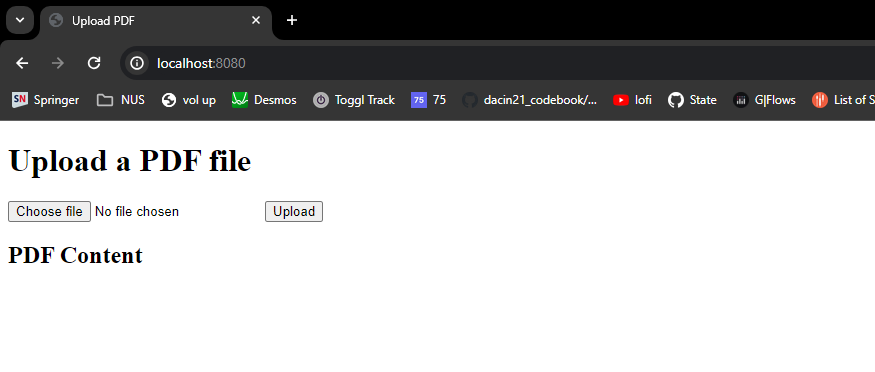
\includegraphics[width=\linewidth/2]{original.png}
\subsection{Uploading}
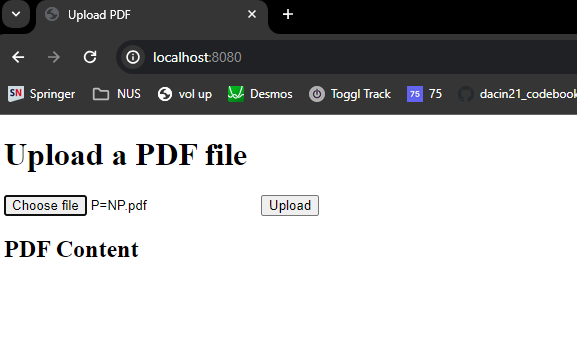
\includegraphics[width=\linewidth/2]{choosefile.png}
\subsection{Uploaded}
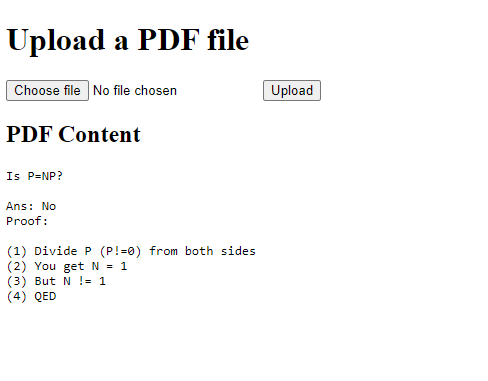
\includegraphics[width=\linewidth/2]{uploadedfile.png}



\end{multicols*}
\end{document}
